This section calibrates and validates the duration-dependent damage function (Eq.~\ref{eq: duration richards}) using a large-scale dataset of real flood insurance claims.

\subsection{Data: FEMA NFIP Flood Insurance Claims}
\label{ssec: fema data}

We use the FEMA National Flood Insurance Program (NFIP) Redacted Claims dataset, accessed via the OpenFEMA API.\footnote{\url{https://www.fema.gov/api/open/v2/FimaNfipClaims}} This dataset contains individual flood insurance claims with reported water depth (in inches), payout amounts, coverage limits, building type, and geographic identifiers. We extract claims from three major US hurricanes with distinct flooding durations:

\begin{table}[h!]
\centering
\resizebox{\textwidth}{!}{
\begin{tabular}{|l|c|c|c|c|c|}
\hline
\textbf{Event} & \textbf{Year} & \textbf{Claims} & \textbf{Valid} & \textbf{Median DR} & \textbf{Typical $\tau$} \\
\hline
Hurricane Sandy & 2012 & 144,848 & 92,283 & 0.190 & 36h \\
Hurricane Harvey & 2017 & 92,398 & 63,642 & 0.428 & 288h \\
Hurricane Katrina & 2005 & 208,348 & 139,712 & 0.627 & 120h \\
\hline
\textbf{Total} & & \textbf{445,594} & \textbf{295,637} & & \\
\hline
\end{tabular}}
\caption{FEMA NFIP claims used for calibration (OpenFEMA snapshot 2026-05-09). ``Valid'' denotes claims with positive water depth, positive payout, positive coverage, and damage ratio in $(0, 1.5]$, capped at 1.0. Damage ratio = total payout / total coverage. Typical duration $\tau$ assigned from FEMA flood extent reports and hydrological literature. The earlier preprint version used a Mar 2026 OpenFEMA snapshot containing 354{,}413 raw / 317{,}943 valid claims; FEMA has since retroactively backfilled $\sim$91{,}000 historical claims, the majority of which lack a recorded water depth and therefore fail the validity filter. The full filter funnel from the 445{,}594 raw records to the 295{,}637 valid records is reported in Appendix~\ref{app: funnel}.}
\label{tab: fema data}
\end{table}

The damage ratio is computed as \[\text{DR} = \frac{\text{building payout} + \text{contents payout}}{\text{building coverage} + \text{contents coverage}},\] clipped to $[0, 1]$. The USACE depth-damage function for one-story residential structures~\cite{usace2003} serves as an instantaneous ($\tau = 0$) anchor.

The three events span a wide range of flooding mechanisms: Sandy was a tidal storm surge with rapid recession ($\sim$36~hours); Harvey was unprecedented rainfall-driven flooding that persisted for over two weeks ($\sim$288~hours); Katrina involved levee breaches with extreme depths but intermediate duration ($\sim$120~hours). This variation enables joint calibration of the duration parameters.

\subsection{Joint Calibration}
\label{ssec: joint calibration}

We calibrate the seven parameters of Eq.~\ref{eq: duration richards} jointly across all three events plus the USACE anchor, using differential evolution~\cite{storn1997differential} (\texttt{seed=42}, \texttt{maxiter=1000}, \texttt{tol=1e-10}) to minimise the weighted sum of squared residuals on binned depth-damage data (12 equal-width bins per event, minimum 10 claims per bin). To match each event's empirical depth distribution, we cap the calibration data at 4\,m for Sandy and Harvey (encompassing $>99.99\%$ of valid claims; Sandy 99.5th percentile = 2.4\,m, Harvey 99.5th percentile = 1.1\,m) and at 10\,m for Katrina ($>99.93\%$; 99.5th percentile = 7.3\,m); this preserves the small Katrina levee-breach tail above 6\,m, which is the data subset that most distinguishes Katrina from the shorter-duration events. Across all three events, 295{,}400 of 295{,}637 valid claims (99.92\%) enter the binned fit. The choice of 12 bins balances resolution against noise; robustness to the binning choice is assessed below (Section~\ref{ssec: validation}).

\begin{equation*}
    \hat{\theta} = \argmin_\theta \sum_{e \in \mathcal{E}} w_e \sum_{i=1}^{n_e} \frac{\left(\overline{\text{DR}}_{e,i} - \DF(h_{e,i}, \tau_e; \theta)\right)^2}{\sigma_{e,i}^2} + \mathcal{R}(\theta)
    %\label{eq: calibration objective}
\end{equation*}
%
where $\mathcal{E} = \{\text{USACE}, \text{Sandy}, \text{Harvey}, \text{Katrina}\}$, $w_{\text{USACE}} = 3$ (upweighted as the only $\tau = 0$ reference), $\sigma_{e,i} = \max(\text{std}_{e,i} / \sqrt{n_{e,i}}, 0.015)$ for the three event panels and $\sigma = 0.03$ uniformly for the USACE anchor, and $\mathcal{R}(\theta)$ is a weak Gaussian regulariser with priors $B \sim \mathcal{N}(3, 3)$, $Q_0 \sim \mathcal{N}(1, 1)$, $a_0 \sim \mathcal{N}(0.5, 0.2)$, $\nu_0 \sim \mathcal{N}(0.5, 0.3)$ and improper (uniform) priors on the duration coefficients $\lambda_a, \lambda_Q \in [0, 3]$, $\delta_\nu \in [0, 2]$. Bounds on the static parameters are $B \in [0.5, 12]$, $Q_0 \in [0.05, 5]$, $a_0 \in [0.1, 0.9]$, $\nu_0 \in [0.1, 3]$. The optimised parameters are:

\begin{table}[h!]
\centering
\begin{tabular}{|c|c|l|}
\hline
\textbf{Parameter} & \textbf{Value} & \textbf{Interpretation} \\
\hline
$B$ & 5.65 & Steepness of damage curve \\
$Q_0$ & 3.45 & Initial threshold asymmetry \\
$a_0$ & 0.54 & Inflection point at $\tau = 0$ \\
$\nu_0$ & 2.61 & Derivative asymmetry at $\tau = 0$ \\
$\lambda_a$ & 0.49 & Inflection shift rate with duration \\
$\lambda_Q$ & $\approx 0$ & Onset speed (not significant) \\
$\delta_\nu$ & $\approx 0$ & Asymmetry growth (not significant) \\
\hline
\end{tabular}
\caption{Calibrated parameters. The optimiser sets $\lambda_Q \approx 0$ and $\delta_\nu \approx 0$, indicating that duration affects damage primarily through inflection point shift, not curve shape change. The four base Richards parameters $(B, Q_0, a_0, \nu_0)$ are non-uniquely identified within the bin-level loss surface: an approximate ridge connects parameter triplets that produce equivalent $D(h, \tau)$ curves over the calibration domain. Practitioners should refer to $D(h, \tau)$ predictions rather than the four base parameters in isolation.}
\label{tab: calibrated params}
\end{table}

\begin{figure}[h!]
\centering
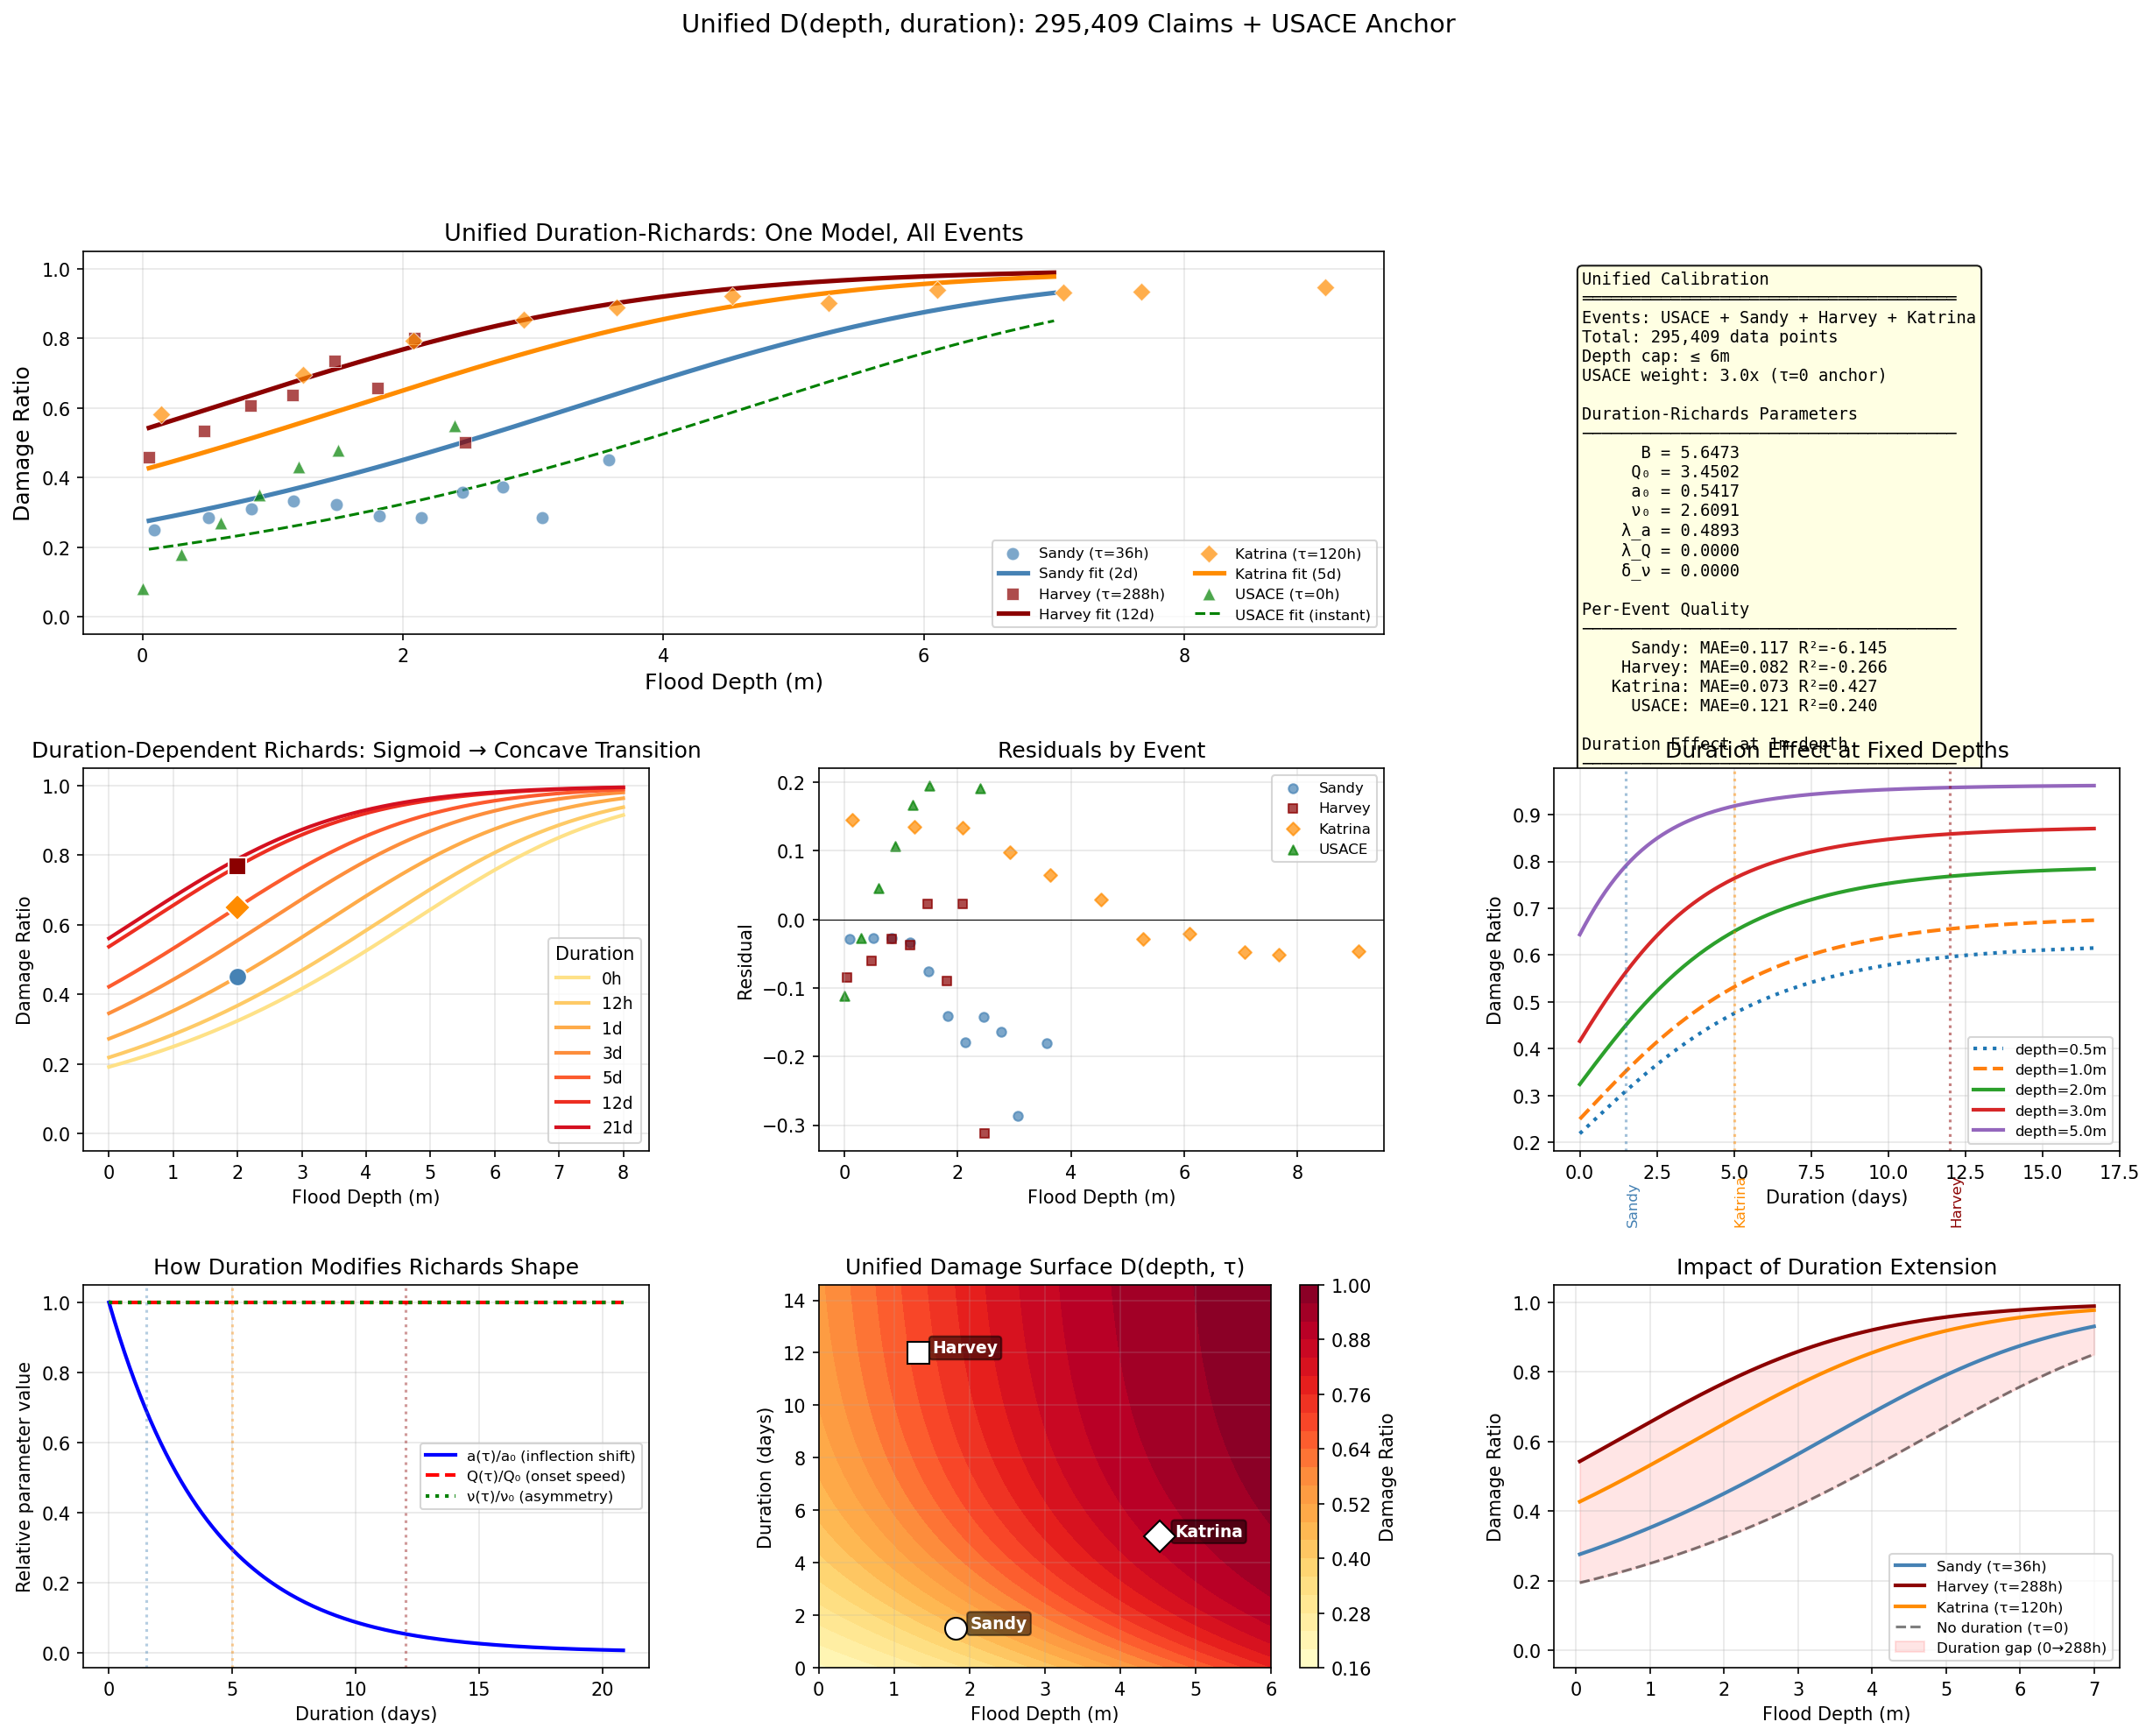
\includegraphics[width=\textwidth]{Content/Images/10_unified_calibration.png}
\caption{Joint calibration across 295{,}637 FEMA claims (295{,}400 used in the binned fit after per-event depth caps and the $\geq 10$ claims-per-bin filter) from three hurricanes plus USACE anchor. Top-left: fitted curves and binned claim means for all events. Bottom-left: duration-dependent transition. Centre: residuals by event. Right panels: parameter evolution with duration and damage surface $D(h, \tau)$. Sandy ($\tau = 36$\,h) is systematically overpredicted; this reflects the compromise of fitting a single $\lambda_a$ across three events with durations spanning an 8 times range. Depth-damage curves are plotted from $h_{\min} = 0.05$\,m.}
\label{fig:unified_calibration}
\end{figure}

\paragraph{Key finding: duration operates through inflection shift only}
Of the three duration-modification channels ($\lambda_a$, $\lambda_Q$, $\delta_\nu$), only $\lambda_a = 0.49$ is significantly non-zero. This means that prolonged flooding shifts the ``50\% damage depth'' toward shallower water, but the fundamental \textit{shape} of the damage curve remains Richards-sigmoidal. This result supports a universality hypothesis: the mechanism of water-induced structural degradation is universal, but the threshold at which it becomes significant depends on exposure time.

At 1~m flood depth, the calibrated model predicts $\text{DR} = 0.25$ for instantaneous flooding, $\text{DR} = 0.35$ at $\tau = 36$~h (Sandy-like), and $\text{DR} = 0.66$ at $\tau = 288$~h (Harvey-like) -- a \textbf{2.6$\times$ increase attributable solely to duration}.

\subsection{Validation}
\label{ssec: validation}

We evaluate the calibrated model through four complementary tests.

\paragraph{Test 1: Leave-one-event-out cross-validation}
We train on two events plus USACE and predict the held-out third event. Table~\ref{tab: loo results} reports the results.

\begin{table}[h!]
\centering
\small
\begin{tabular}{|l|c|c|c|}
\hline
\textbf{Held-out event} & \textbf{Our MAE} & \textbf{USACE MAE} & \textbf{Improv.} \\
\hline
Katrina & 0.435 & 0.523 & +17\% \\
Harvey (from Sandy+USACE) & 0.301 & 0.376 & +20\% \\
\hline
\end{tabular}
\caption{Leave-one-event-out validation. The duration-extended model improves over USACE by 17--20\% when extrapolating to unseen events.}
\label{tab: loo results}
\end{table}

\paragraph{Test 2: Within-event stability and binning sensitivity}
Random 70/30 train-test splits within each event, repeated 5 times, yield MAE = $0.215 \pm 0.001$ (Sandy), $0.294 \pm 0.001$ (Harvey), $0.306 \pm 0.001$ (Katrina). The near-zero variance across splits confirms model stability. We also verify sensitivity to the binning choice: recalibrating with 8 and 16 bins per event (minimum 10 claims per bin enforced) changes the calibrated parameters by less than 3\% and the Harvey MAE by less than 0.005, confirming that the key results are not artefacts of the 12-bin choice.

\paragraph{Test 3: Benchmark against JRC/CLIMADA}
We compare predicted damage ratios against the JRC Global Flood Depth-Damage Functions~\cite{huizinga2017global}, which underpin CLIMADA's flood impact module~\cite{aznar2019climada}. Using Harvey binned data as ground truth:

\begin{table}[h!]
\centering
\begin{tabular}{|l|c|c|}
\hline
\textbf{Model} & \textbf{MAE} & \textbf{Bias} \\
\hline
Duration-Richards ($\tau = 120$h) & \textbf{0.108} & $+0.012$ \\
Duration-Richards ($\tau = 288$h) & 0.095 & $-0.095$ \\
JRC Residential (North America) & 0.214 & $+0.153$ \\
USACE Reference & 0.288 & $+0.288$ \\
\hline
\end{tabular}
\caption{Benchmark against JRC/CLIMADA on Harvey binned data. Bias = actual $-$ predicted; positive values indicate underprediction. JRC underpredicts by $\sim$0.15 because it lacks a duration parameter. Our model reduces MAE by about 50\%.}
\label{tab: climada benchmark}
\end{table}

The JRC curves systematically underpredict Harvey damage: at 1~m depth, JRC predicts $\text{DR} \approx 0.40$ while actual Harvey claims show $\text{DR} \approx 0.55$, a gap of about 15 percentage points (Bias column reports actual $-$ predicted). This gap is largely attributable to the absence of a duration parameter, though differences in construction standards and claim-processing practices between the JRC reference sample and NFIP data may also contribute.

\paragraph{Test 4: Correlation with financial distress proxies}
Using FEMA Individual and Household Program (IHP) registrations for Harvey (301 ZIP codes with $\geq$20 registrations), we test whether predicted damage ratios correlate with real financial distress outcomes:

\begin{table}[h!]
\centering
\begin{tabular}{|l|c|c|}
\hline
\textbf{Distress proxy} & \textbf{Spearman $\rho$} & \textbf{$p$-value} \\
\hline
Mean FEMA damage amount (\$) & 0.949 & $< 0.001$ \\
\% properties with flood damage & 0.904 & $< 0.001$ \\
Mean IHP assistance payment (\$) & 0.885 & $< 0.001$ \\
\% SBA disaster loans approved & 0.345 & $< 0.001$ \\
\hline
\end{tabular}
\caption{Spearman rank correlation between ZIP-level predicted damage ratio and real financial distress proxies ($n = 301$ ZIP codes).}
\label{tab: defaults correlation}
\end{table}

The near-perfect rank correlation ($\rho = 0.949$) with actual damage amounts confirms that the model correctly orders geographic areas by risk severity. Quintile analysis shows monotonic increase: ZIP codes in the highest predicted-risk quintile experienced 14$\times$ higher mean damage (\$16.9K) than the lowest quintile (\$1.2K).

\subsection{Feature enrichment analysis}
\label{ssec: feature enrichment}

To assess the potential for improving individual-claim prediction accuracy, we compare the depth-only Richards model against progressively enriched models using building characteristics available in the NFIP dataset (Harvey, 70/30 split):

\begin{table}[h!]
\centering
\begin{tabular}{|l|c|c|c|}
\hline
\textbf{Model} & \textbf{MAE} & \textbf{R$^2$} & \textbf{$\Delta$ MAE vs M0} \\
\hline
M0: $\DF(\text{depth})$ & 0.250 & 0.046 &  --  \\
M1: + occupancy type & 0.250 & 0.055 & $-0.1$\% \\
M2: + number of floors & 0.245 & 0.080 & $-2.3$\% \\
M3: + basement indicator & 0.244 & 0.086 & $-2.4$\% \\
M4: Gradient boosting (all) & 0.221 & 0.217 & $-11.7$\% \\
\hline
\end{tabular}
\caption{Feature enrichment on Harvey claims (44K train, 19K test). Gradient boosting feature importance: depth 74\%, occupancy 11\%, floors 6\%, primary residence 5\%, basement 3\%.}
\label{tab: feature enrichment}
\end{table}

Flood depth alone accounts for 74\% of the gradient boosting model's predictive power. Building characteristics add 17 percentage points of explained variance but reduce MAE by only 11.7\%. The residual MAE $\approx 0.22$ likely represents an irreducible noise floor arising from the bimodal distribution of individual claim outcomes. For portfolio-level credit risk assessment, where individual errors average out, the depth-only Duration-Richards model provides adequate accuracy.
